\hfill\newline
%will take care of tex and graphs when the body is finished
%should ask for more experimental details
%revise the sentences!
\phantom{ } The circuit in Figure[\ref{fig:cir}] was built again to measure the response to a sinusoidal input. Channel 1 and 2 were connected into the circuit to display the voltage over the input port and the capacitor. Figure[\ref{fig:sinwave}] shows the waveform of these two voltages, as captured from the oscilloscope display. 

\begin{figure}[!htbp]
	\centering
	\begin{framed}
	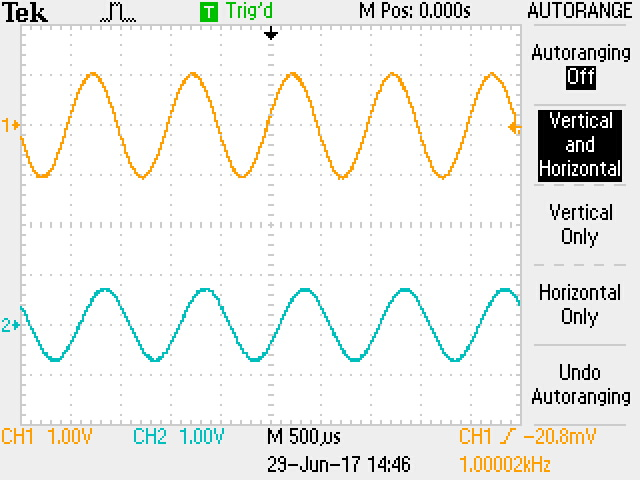
\includegraphics[width=\linewidth]{images/TEK0011.JPG}
	\caption{Waveform of input and output voltages}
		\end{framed}
	\label{fig:sinwave}
\end{figure}

\phantom{ } To measure the response to signals of various frequencies, we kept the input amplitude at 1V, and swept the input frequency from 10Hz to 1MHz. Table[\ref{tab:caf}] shows the recorded amplitudes of the output signals. Figure[\ref{fig:caf}] is a plotted figure of the amplitude-frequency data, with a logarithmic scale on the x-axis.

\begin{table}[!htbp]
	\centering
	\caption{Experiment record of amplitude over the capacitor}
	\begin{tabular}{lccllcc}
		\toprule
		No&freq(Hz)&Amp(V)&&No&freq(Hz)  &Ampe(V)\\
		\midrule
		1	&10		&1040	&&9 &$5*10^3$&240\\
		2	&20		&1040	&&10&$1*10^4$&160\\
		3	&50		&1040	&&11&$2*10^4$&120\\
		4	&100	&1040	&&12&$5*10^4$&80\\
		5	&200	&1040	&&13&$1*10^5$&23.2\\
		6	&500	&920	&&14&$2*10^5$&16.8\\
		7	&1000	&720	&&15&$5*10^5$&13.6\\
		8	&2000	&480	&&16&$1*10^6$&12.8\\
		\bottomrule
	\end{tabular}
	\label{tab:caf}
\end{table}

\begin{figure}[!htbp]
	\centering
	\begin{framed}
	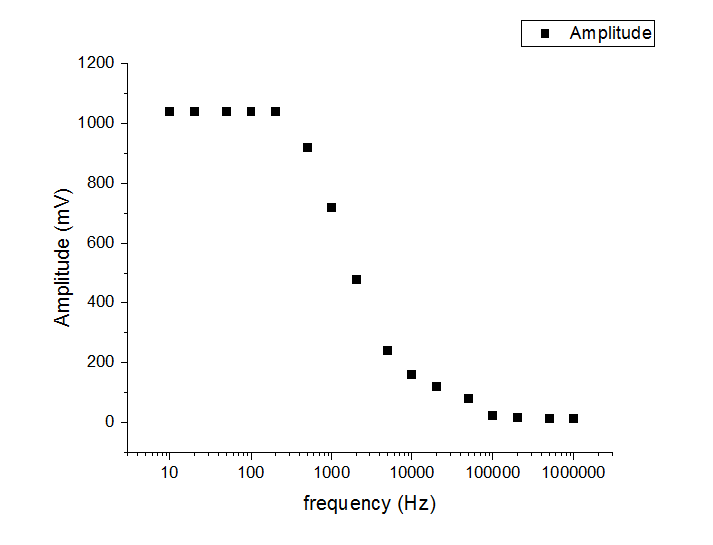
\includegraphics[width=\linewidth]{images/c-amp-freq.png}
	\caption{Voltage over the capacitor in terms of frequency}
		\end{framed}
	\label{fig:caf}
\end{figure}

\hfill \newline
\textbf{Analysis \#6:} \newline
\phantom{ } Comparing the figure above to what was plotted in prelab\#11, we noticed that the pattern of data we collected in the experiment was consistent with the calculation before. Amplitude decreased rapidly with the frequency increasing in middle range, while the slope was comparatively small with the frequency approaching $10^6$. However, the curve between $10^4$ and $10^5$ was not very smooth. The error may has occurred with the oscilloscope. We noticed that sometimes moving the cursor on the time axis makes no difference. The reason might be that the machine measures its display to give out values, which means an unavoidable error from the width of the lines. \\
\phantom{ } Next, we changed the output to be the voltage over the resistor, and the function generator to provide a sinusoidal wave with 1V amplitude. Table[\ref{tab:raf}] shows the amplitudes recorded under various frequencies, and they are plotted in the figure Fig[\ref{fig:raf}].

\begin{table}[!htbp]
	\centering
	\caption{Experiment record of amplitude over the resistor}
	\begin{tabular}{lccllcc}
		\toprule
		No&freq(Hz)&Amp(mV)&&No&freq(Hz)  &Amp(mV)\\
		\midrule
		1	&10		&22.4	&&9 &$5*10^3$&1020\\
		2	&20		&30.4	&&10&$1*10^4$&1060\\
		3	&50		&72.0	&&11&$2*10^4$&1060\\
		4	&100	&124	&&12&$5*10^4$&1060\\
		5	&200	&224	&&13&$1*10^5$&1060\\
		6	&500	&480	&&14&$2*10^5$&1060\\
		7	&1000	&740	&&15&$5*10^5$&1060\\
		8	&2000	&940	&&16&$1*10^6$&1060\\
		\bottomrule
	\end{tabular}
	\label{tab:raf}
\end{table}

\begin{figure}[!htbp]
	\centering
	\begin{framed}
	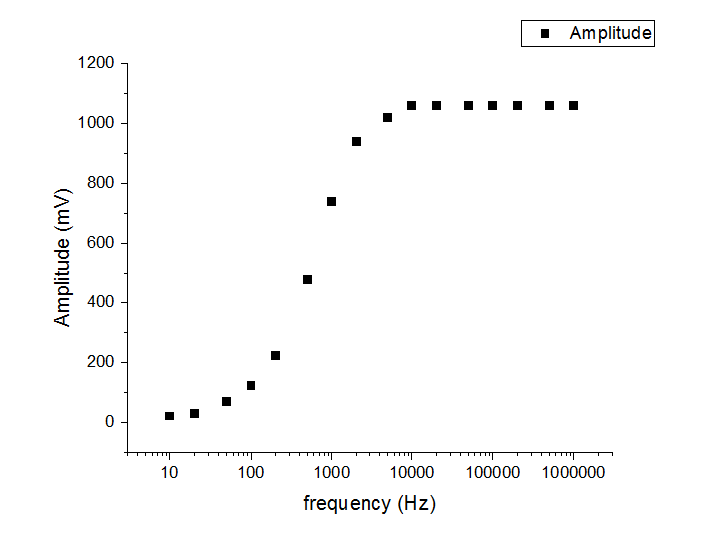
\includegraphics[width=\linewidth]{images/r-amp-freq.png}
	\caption{Voltage over the resistor in terms of frequency}
		\end{framed}
	\label{fig:raf}
\end{figure}

\hfill \newline
\textbf{Analysis \#7:} \newline
\phantom{ } The figure above shows no big difference to what was plotted in prelab\#12. They are of the same shape, increasing rapidly with a mid-range frequency, and become close to horizontal after $10^4$. A slight error might have been caused by working principles of the instrument, as mentioned before.